\documentclass{article}
\usepackage{polski}
\usepackage{graphicx}
\usepackage{subcaption}

\title{Drony w edukacji}
\author{Szymon Przepióra}

\begin{document}

\maketitle
\pagenumbering{gobble}
\newpage
\pagenumbering{arabic}

\section{Co to jest dron ?}

Drony czyli tak naprawdę bezzałogowe statki powietrzne, stają się ostatnio coraz bardziej popularne nie tylko w celach rozrywkowych i rekreacyjnych ale również odgrywają ważną rolę w wielu dziedzinach nauki.
 W tym artykule omówię zastosowanie dronów w szeroko rozumianej edukacji szkolnej na podstawie drona DJI Ryze Tello.

\begin{figure}[h!]
  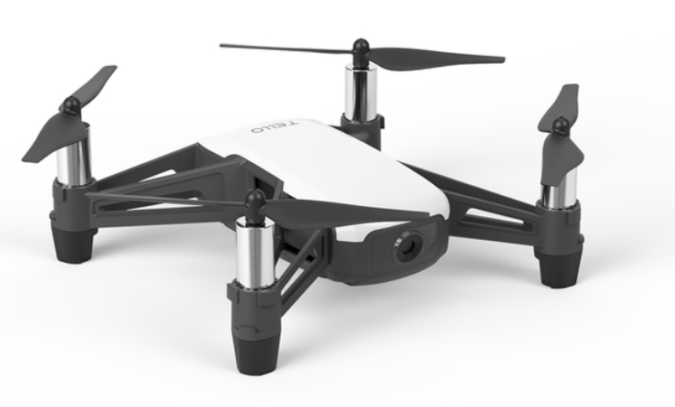
\includegraphics[width=\linewidth]{tello.jpg}
  \caption{DJI Ryze Tello}
  \label{fig:tello1}
\end{figure}

Należy zacząć od wyjaśnienia, czym jest dron. To bezzałogowy statek powietrzny pilotowany zdalnie lub wykonujący lot autonomicznie, czyli samodzielnie.
 Spotykany jest również pod nazwami (ang. unmanned aerial vehicle, UAV) lub (ang. unmanned aerial system, UAS).

\section{Gdzie i czym można latać ?}
Na terenie kraju w celach niekomercyjnych, bez specjalnego zezwolenia i z zachowaniem zasad ostrożności (zachowanie odpowiedniej odległości od ludzi i budynków) można latać małymi dronami o wadzę do 0,6 kg, do wysokości 30 m od ziemi lub do wysokości najwyższej przeszkody terenowej, takiej jak na przykład drzewa, w promieniu do 100m od operatora. Ryze Tello mieści się w tej kategorii.

Licencji nie wymaga również sterowanie dużymi dronami o wadzę całkowitej nie przekraczającej 25 kg, pozostając z nim w stałym kontakcie wzrokowym w niekontrolowanie przestrzeni powietrznej (klasa G).

Żeby użyj drona do celów edukacyjnych potrzebujemy specjalnego świadectwa kwalifikacji UAVO. Zdobyć je można po przejściu badań lekarskich, wykupieniu ubezpieczenia OC i zdania egzaminu państwowego. 

\section{Programowanie dronów.}
Programowanie drona DJI Ryze Tello odbywa się przy pomocy programu DroneBlocks. Jest on stworzony na podstawie języka programowania Scratch, który powstał jako środek do nauczania dzieci i młodzieży podstaw programowania. Samo pisanie kodu odbywa się w sposób wizualny przy pomocy klocków z danymi działaniami. Język ten już dzisiaj jest stosowany w wielu szkołach jako wstęp do programowania.  Co ułatwia przejście na zajęciach z jednego środowiska do drugiego.


\begin{figure}[h!]
  \centering
  \begin{subfigure}[b]{0.4\linewidth}
    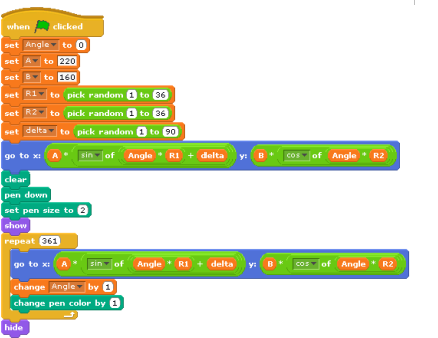
\includegraphics[width=\linewidth]{kod2.jpg}
    \caption{język Scratch.}
  \end{subfigure}
  \begin{subfigure}[b]{0.4\linewidth}
    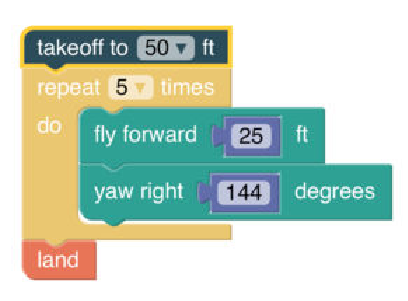
\includegraphics[width=\linewidth]{kod1.jpg}
    \caption{język DroneBlocks.}
  \end{subfigure}
  \caption{Przykładowe programy.}
  \label{fig:coffee}
\end{figure}

Drony są bardzo przydatne do pokazania uczniom jak działają podstawowe operacje w programowaniu, takie jak na przykład pętla, elementy logiczne oraz porównania. Są one w stanie pokazać oddziaływanie napisanego kodu na świat rzeczywisty co bez takich narzędzi jest problematyczne. 
Dzięki programowaniu uczniowie są również w łatwy sposób zaprogramować ruchy drona, które bez kody były by bardzo trudne do wykonania nawet dla zaawansowanego operatora.

\section{Zastosowania w szkołach.}

\subsection{Fizyka i matematyka.}

Drony można użyć również podczas zajęć matematyki lub fizyki. Przedmioty te mogą sprawiać trudności uczniom ponieważ brak zastosowania w praktyce sprawia, że są tak abstrakcyjne. Przy pomocy dronów uczniowie są w stanie zobaczyć jak wzory, które obliczają na zajęciach przekładają się na rzeczywisty ruch. Daje to również nowe możliwości dla nauczycieli, którzy mogą zadawać nowe bardziej wymagające zadania takie jak obliczanie jak wiatr ma wpływ na ruch drona lub obliczanie ile dronowi zajmie przelecenia danego odcinka. Opcji jest bardzo wiele i zależą jedynie od nauczyciela prowadzącego przedmiot.

\subsection{Geografia}




\end{document}

